\chapter{VectorHelmholtz -- model wave propagation in bent waveguide}
\label{vectorhelmholtz-bent-waveguide-chapt}

\modinfo{Directory}{WaveguideGUI}
\modinfo{Solvers}{\Idx{VectorHelmholtz}} 
\modinfo{Tools}{\Idx{ElmerGUI}} 
\modinfo{Dimensions}{3D, Steady-state}
\modinfo{Author}{Juhani Kataja}


\subsection*{Case definition}

In this tutorial we model propagation of a guided wave through a bend in a rectangular waveguide.  Let us choose the primary wave to be a $TE_{10}$ mode at $f=2.5~ \mathrm{GHz}$ propagating in the positive $z$ axis direction (time-harmonic convention $e^{-i\omega t}$).

\begin{wrapfigure}{r}{0.5\textwidth}
\centering
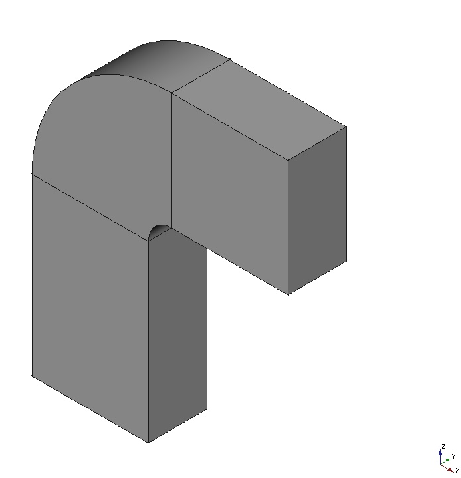
\includegraphics{geom.pdf}
\caption{Geometry of the waveguide}
\label{fig:geometry}
\end{wrapfigure}

The electric field of the primary wave is given by \[ \vec E_p = \vec u_y \frac{ik}{k_c}\sin(k_cx)e^{i\beta z},\] where $k_c = \pi / a$, $k = \omega \sqrt{\varepsilon_0 \mu_0}$ and $\beta = \sqrt{k^2-k_c^2}$. The dimensions of the waveguide's cross section are $a=10~ \mathrm{cm}$ and $b=5~ \mathrm{cm}$, the bend is a piece of circular torus with outer radius of $12~ \mathrm{cm}$ and inner radius of $2~ \mathrm{cm}$. The waveguide geometry is depicted in Fig.~\ref{fig:geometry}.

The input port is that part of the boundary which is normal to $z$ -axis, the output port that which is normal to $x$ -axis and the rest of the boundary is a PEC boundary.

The PEC boundary condition is given by $\vec n \times \vec E = 0$, the input boundary condition by
\[\vec n \times \nabla \times \vec E - i\beta \vec n \times 
        (\vec n \times \vec E) = i2\beta \vec n \times 
                                     (\vec n \times \vec E_p),\]
and the output boundary condition by \[\vec n \times \nabla \times \vec E - i\beta \vec n \times (\vec n \times \vec E)=0.\] Here $\vec n$ is the exterior normal of the domain.

\subsection*{Load ElmerGUI Equation Menu}

The GUI definitions of VectorHelmholtz solver utilized in this tutorial are located in the \texttt{edf-extra} folder and thus need to be manually activated in the ElmerGUI.\\

Note that the extra definition needs to be loaded first, before any other steps in building any tutorial.  Once the extra definition has been loaded, and the ElmerGUI project has been saved, then the instructions for the extra definition will be stored in the project, and you won't have to load the extra definition again.

\begin{verbatim}
File
  Definitions
    Append -> vectorhelmholtz.xml
  Close
\end{verbatim}

The \texttt{\Idx{vectorhelmholtz.xml}} definition file is, by default, located in Linux in:

\texttt{\$ELMER\_HOME/share/ElmerGUI/edf-extra}\\

and in Windows, located in:

\texttt{C:/Program Files/Elmer 9.0-Release/share/ElmerGUI/edf-extra}\\

We will also be using the \Idx{Result Output Solver}, which is one of the default, pre-loaded GUI definitions, so it does not need to be manually activated.  For reference, the  \texttt{\Idx{resultoutput.xml}} definition file is, by default, located in Linux in:

\texttt{\$ELMER\_HOME/share/ElmerGUI/edf}\\

and in Windows, located in:

\texttt{C:/Program Files/Elmer 9.0-Release/share/ElmerGUI/edf}\\

After reading over several of the preceding tutorials that wrote results to the \texttt{case.vtu} file, and none of those tutorial used Result Output Solver, you may be wondering why we now all of a sudden need to load a special solver to output results?\\

Actually, the Result Output Solver has been loaded in each of the preceding tutorials, but it was done in the background, without notifying the user.  All one needs to do, is to enter a file name into the Post file field in the Setup menu, as follows.

\begin{verbatim}
Model
  Setup
    Post file -> case.vtu
  Apply
\end{verbatim}

This will cause Result Output Solver to be loaded in the background and will run after saving the simulation.  To get back to your question, why add an equation entry for Result Output, the answer will be that we want to demonstrate how to use some of the advanced features of the Result Output Solver.  Please take a look at the Elmer Models Manual and review the Result Output Solver.  One of the features that we will use, is to ask for the .vtu file to be output in ASCII, instead of in binary.\\

Another feature of Result Output Solver is the ability to save the results in formats other than .vtu, including vtk, Dx, Gmsh, and GiD formats.\\

One last point, either enter a `case.vtu' name into the Post file field of Setup, or add Result Output Solver to an Elmer project.  Don't add both, it won't hurt anything, but it will output two .vtu files, one will be valid and the other will be empty.\\

\subsection*{ElmerGUI Solution Procedure}

Load geometry:
\begin{verbatim}
File
  Open -> waveguide_bend.step
\end{verbatim}

As we are modelling a wave phenomenon at $2.5 \mathrm{GHz}$ the maximum H (maximum element size) in the mesh must be around $\frac 1 {10\lambda}$, where $\lambda\approx8.3$, so set Max H = 0.012.  We mentioned the waveguide cross section is 10 cm by 5 cm, which equals 0.100 meters by 0.050 meters.  Taking the smaller dimension and dividing by Max H, gives 0.050/0.012 = approximately four elements across the smaller dimension.\\

Within ElmerGUI, since the geometry input file is in Step format, Nglib from Netgen is used to mesh the model into linear tetrahedral elements.  Nglib by default will generate a mesh where at least two elements will span the smaller dimension of the model.  In this case, setting Max H = 0.012 to obtain about four elements across the smaller dimension is a necessary step.\\

Note that one could use Elmergrid to increase the order of the tet mesh generated by nglib from linear to quadratic, (from a command prompt, enter elmergrid 2 2 -increase) although in this case we keep the linear mesh as generated by nglib.

\begin{verbatim}
Mesh
  Configure..
    Max H: 0.012
    Apply
Mesh
  Remesh
\end{verbatim}

Add the \texttt{VectorHelmholtz} and \texttt{VectorHelmholtzCalcFields} solver modules:
\begin{verbatim}
Model
  Equation -> Add..
    Vector Helmholtz Post Process
      Active = on
      Priority 4
    Result Output
      Active = on
      Priority 2
        Edit solver settings
          Solver specific options
            Uncheck the box `Binary Output'
         Apply
    Vector Helmholtz Equation
      Active = on
      Apply to Bodies: Body 1
      Angular Frequency = $ 2*pi*2.5e9
      Priority 5
      Free text input
        $ a = 10e-2
        $ b = 5e-2
        $ c0 = 1/sqrt(8.854e-12*4*pi*10^-7)
        $ omega=2*pi*2.5e9
        $ k0 = omega/c0
        $ kc = pi/a
        $ beta0 = sqrt(k0^2-kc^2)
      Edit Solver Settings
        Linear system
          Iterative = BiCGStabl
          Preconditioning = vanka
          BiCGStabl order = 6
          Convergence tol = 1e-6
          Apply
      Add
    OK
\end{verbatim}

Here in the \texttt{Free text input} part we defined some constants that will make definition of the rest of the model easier.\\ 

Then add boundary PEC conditions:
\begin{verbatim}
Model
  Boundary Condition -> Add..
  Name = PEC
  VectorHelmholtz Equation
    E re {e} = 0
    E im {e} = 0
    Apply to boundaries = 2...13
    Add
  OK
\end{verbatim}

Note that because the mesh is tetrahedral, the \texttt{E re/im \{f\}} Dirichlet condition is unnecessary. The hexahedral and pyramidal Piola transformed elements have DOFs on element faces rendering the \texttt{\{f\}} Dirichlet conditions meaningful.

Add the input port boundary condition:
\begin{verbatim}
Model
  Boundary Condition -> Add..
  Name = Inport
  Apply to boundaries = 14
  VectorHelmholtz Equation
    Magnetic Boundary Load 2 [enter]
      Variable Coordinate 1
      Real MATC "-2*beta0*k0/kc*sin(kc*(tx+a/2))"
      Close
    Electric Robin Coefficient im = $ beta0
  Add
  OK
\end{verbatim}

Next add the output port boundary
\begin{verbatim}
Model
  Boundary Condition -> Add..
  Name = Outport
  Apply to boundaries = 1
  VectorHelmholtz Equation
    Electric Robin Coefficient im = $ beta0
  Add
  OK
\end{verbatim}

Assign material to the body
\begin{verbatim}
Model
  Material -> Add..
  Apply to bodies: Body 1
  Relative Permittivity = 1
  Add
  OK
\end{verbatim}

Now navigate to choose what results are to be saved:
\begin{verbatim}
Model
  Equation -> Equation 1
  Vector Helmholtz Post Process
    Edit Solver Settings
      Solver specific options
        Calculate Electric Field = on
        Calculate Magnetic Field Strength = on
        Calculate Poynting Vector = on
        Calculate Energy Functional = on
        Apply
      Update
      OK
\end{verbatim}

Save the project
\begin{verbatim}
File
  Save project -> [choose location]
\end{verbatim}

And solve:
\begin{verbatim}
Run
  Start Solver
\end{verbatim}

The resulting fields should now appear in \texttt{case0001.vtu} file ready for further post processing.

\subsection*{Results}
We are interested in the \texttt{Energy Functional Value} in the solver log. It should read (prepended with ``\texttt{VectorHelmholtzSolver:}'')

\small{
\begin{verbatim}
Energy Functional value:  -11284.937620324963        453999.53923919413
\end{verbatim}
}

The first number is the real part and second the imaginary part. Denoting this with $l(E)$ it holds that in this case \[l(E) = \frac {i \beta k_0^2 ab}{\mu k_c^2} (1+\rho),\] where $\rho$ is the reflection coefficient of electric field. Thus $\rho\approx-0.022+0.024i$, which translates to roughly $29.7~\mathrm{dB}$ return loss.

In Fig.~\ref{fig:solution} the Poynting vector and the real part of the electric field of the solution field is shown.

\begin{figure}[htbp]
\centering
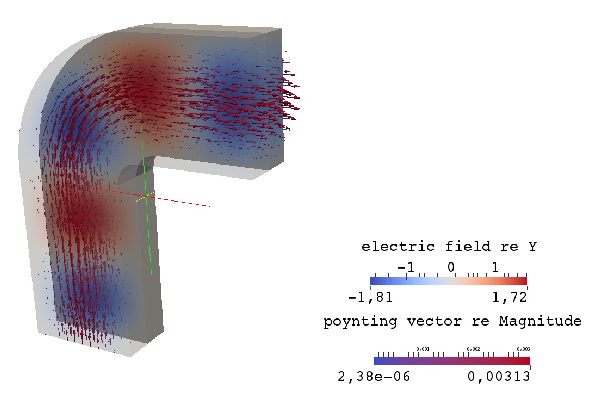
\includegraphics[width=0.8\textwidth]{result.pdf}
\caption{The resulting field solution: The $y$ -component of the real part of the electric field and the real part of Poynting's vector}
\label{fig:solution}
\end{figure}

\subsection*{Extra task:}

Try outputting results using the .vtk format, and loading the .vtk file using Paraview.  Also try saving the results in binary as well as in ASCII, and compare the resulting .vtu files using a text editor.

